\section{Case Study: Large Scale Analysis}

\def \apitotalALL {68,268}
\def \apctotalALL {2,115}

\def \apicountALL {1,471}
\def \apiprcntALL {41.19\%}
\def \apicountZOO {878}
\def \apicountFDR {593}

\def \apccountALL {761}
\def \apcprcntALL {20.05\%}
\def \apccountZOO {464}
\def \apccountFDR {252}

\def \andzooct {2,180}
\def \fdroidct {1,391}

\def \prqcount {224}
\def \prqprcnt {12.34\%}
\def \prqtotal {1,815}

\def \prvcount {1,206}
\def \prvprcnt {68.68\%}
\def \prvtotal {1,756}

In order to evaluate the performance of \@approach under real-world usage, we
downloaded \andzooct\ randomly-selected applications from Androzoo
\cite{allix2016androzoo} and the \fdroidct\ most recently updated apps from
FDroid \cite{fdroid}.  We then analyzed each app using \@approach to assess
whether it can detect potential mismatches within an acceptable time even on
real-world apps. We report our findings in terms of the number of apps from the
population that can suffer from both API and permission mismatches. 

Overall, our experimental results reveal that \@approach takes 6.6 seconds on
average to analyze a single app, ranging from 1.5 seconds to 16.8 seconds. 

We detected \apitotalALL\ potential API invocation mismatches in the population,
with approximately \apiprcntALL\ of the apps harboring at least one potential
mismatch.  Of those vulnerable apps, \apicountZOO\ came from Androzoo and
\apicountFDR\ from FDroid. We also found \apctotalALL\ potential API callback
mismatches occurring in \apcprcntALL of the apps selected, with \apccountZOO\
apps from Androzoo and \apccountFDR\ apps from FDroid exhibiting potential
vulnerability. Most apps had either zero or very few API-related mismatches, as
shown in Figure \ref{fig:clusters}.

\begin{figure}
    \begin{subfigure}{0.48\textwidth}
        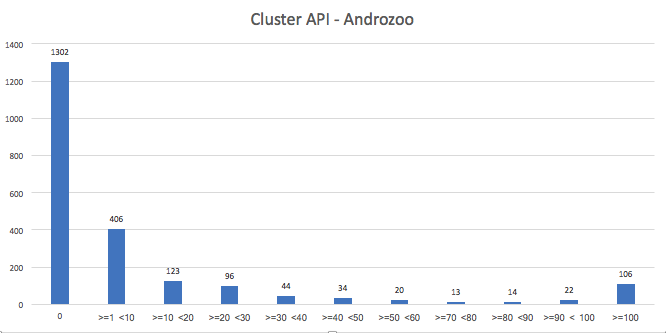
\includegraphics[width=\textwidth]{images/cluster_api_androzoo.png}
    \end{subfigure}
    ~
    \begin{subfigure}{0.48\textwidth}
        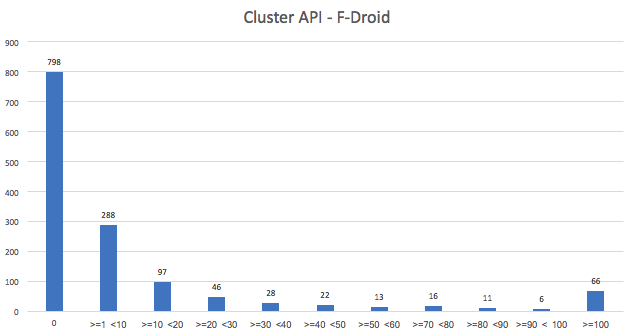
\includegraphics[width=\textwidth]{images/cluster_api_fdroid.png}
    \end{subfigure}
    
        \begin{subfigure}{0.48\textwidth}
        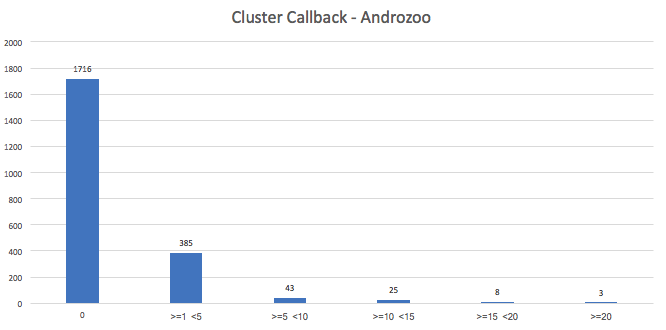
\includegraphics[width=\textwidth]{images/cluster_callback_androzoo.png}
    \end{subfigure}
    ~
    \begin{subfigure}{0.48\textwidth}
        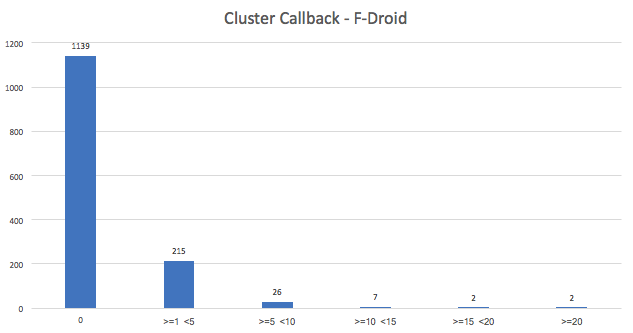
\includegraphics[width=\textwidth]{images/cluster_callback_fdroid.png}
    \end{subfigure}
    \caption{Apps grouped by number of API-related mismatches reported}
    \label{fig:clusters}
\end{figure}

To evaluate permission-related mismatch analysis, we divided the apps into two
groups based on the target SDK version: (i) \prqtotal\ apps target Android API
levels greater than or equal to 23 and (ii) \prvtotal\ apps target Android API
levels below 23. We identified a total of 1,430 apps across both groups
reporting a permissions-related mismatch.

As explained in Section \ref{sec-background:prm}, the first group of apps is
subject to a permissions-related mismatch if the app does not implement the
runtime permissions request system introduced in API level 23. Of the \prqtotal\
apps targeting API levels greater than or equal to 23, \prqcount\ apps
(\prqprcnt) attempt to use dangerous permissions without implementing the
runtime permissions request system. The apps which target levels lower than 23
may encounter a mismatch if they use dangerous permissions which are
subsequently revoked by the user. Of the \prvtotal\ apps in that group,
\prvcount\ apps (\prvprcnt) use the dangerous permissions from their manifest
and are vulnerable to this type of mismatch.

Based on our analysis results, we conclude that our tool can effectively
identify potential API mismatches and permission violations. It also performs
analyses efficiently, allowing it to be used to analyze a large collection of
real-world applications. To illustrate the practical applications of \@approach,
imagine a company that provides its employees with Android smart-mobile devices.
Prior to each platform update, the system administration team could simply apply
our tool on the collection of all the necessary apps needed by the employees to
quickly identify apps that may misbehave when execute in the new platform,
making updates safer and improving the overall user experience.
